Dieses Tutorial / Template ist so aufgebaut, dass in der Datei \menu{Tutorial.tex} alle Struktur-Informationen des Dokumentes enthalten sind. Im wesentlichen sind dies die Reihenfolge aller Kapitel (section) und Unterkapitel (subsection).

\begin{figure}[h!]
\centering
  % 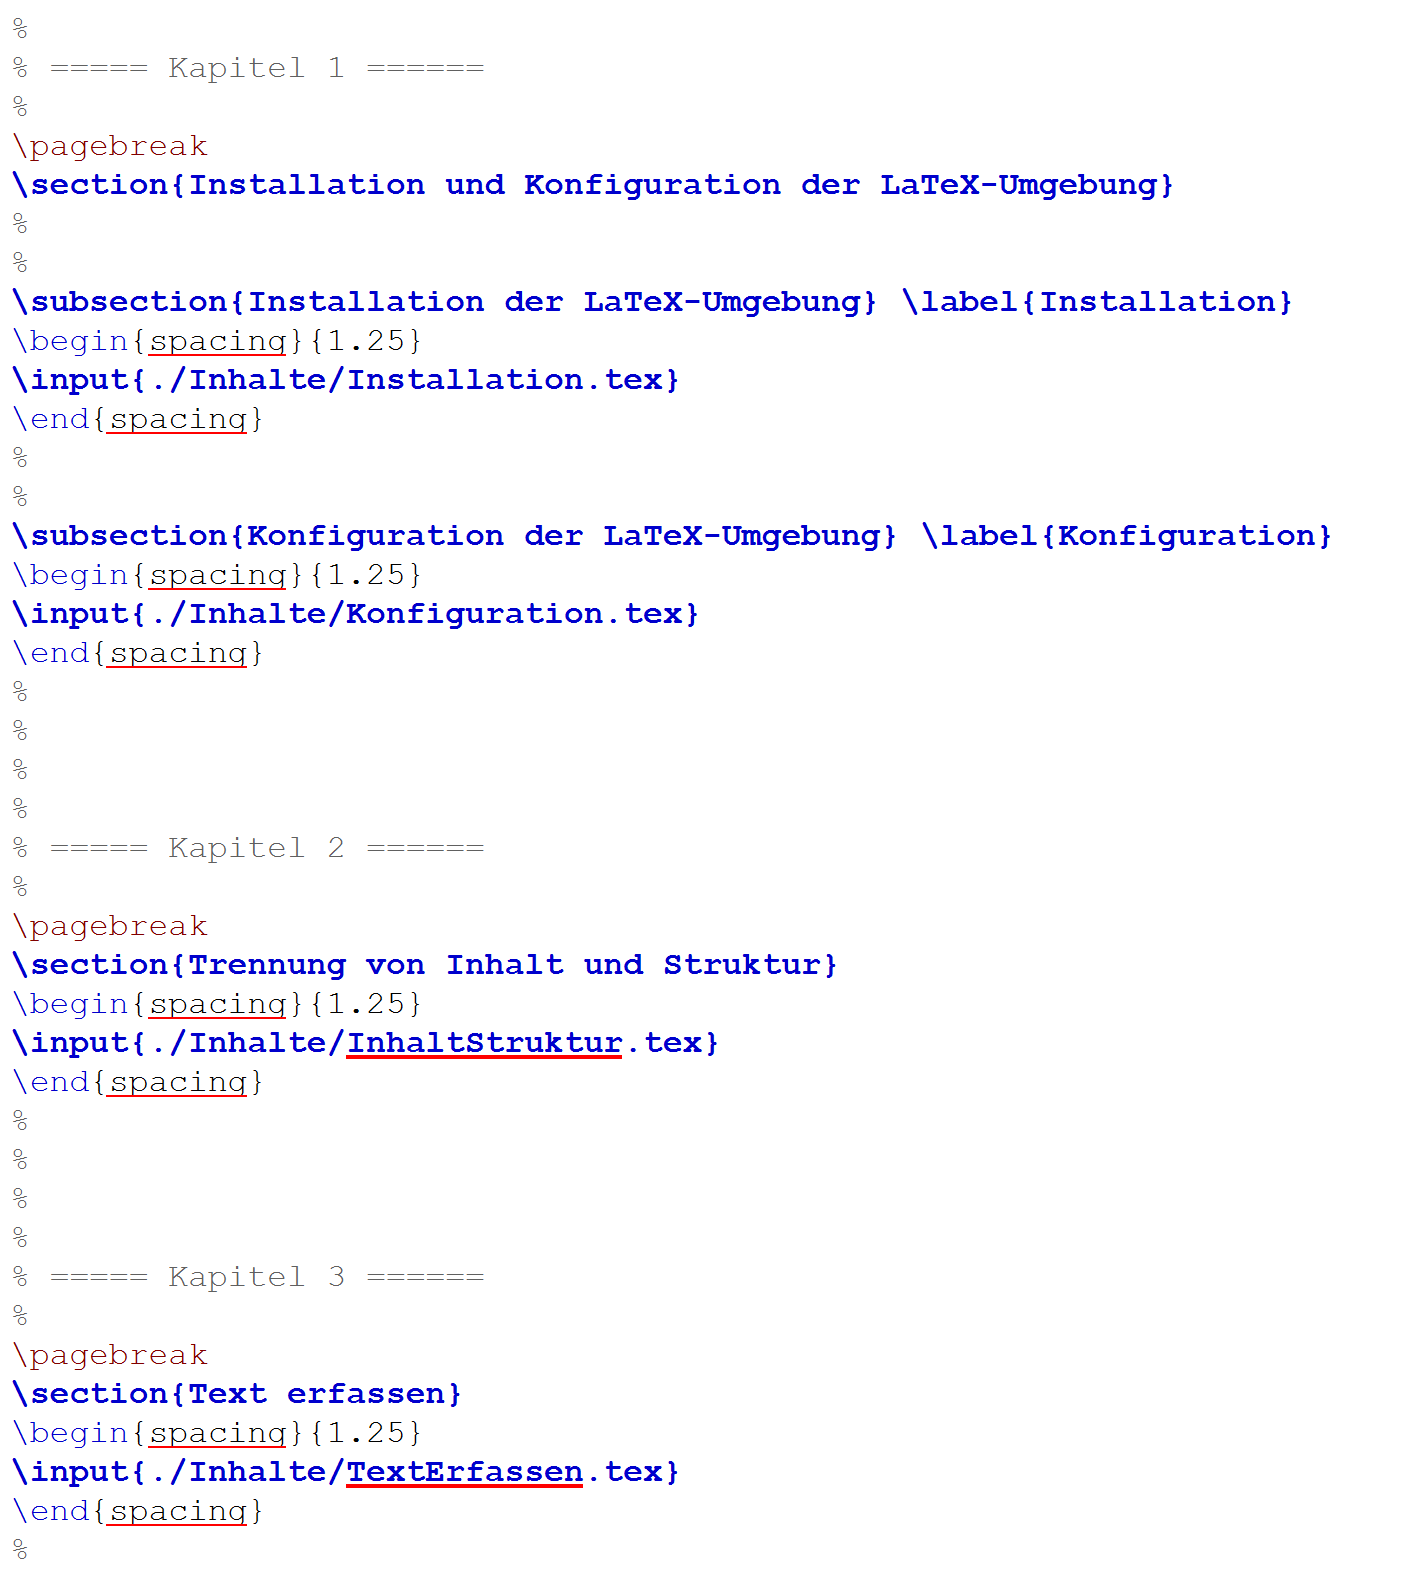
\includegraphics[width=0.9\textwidth]{./Bilder/TextStruktur_1.png}        % Bild ohne Rahmen
  \fbox{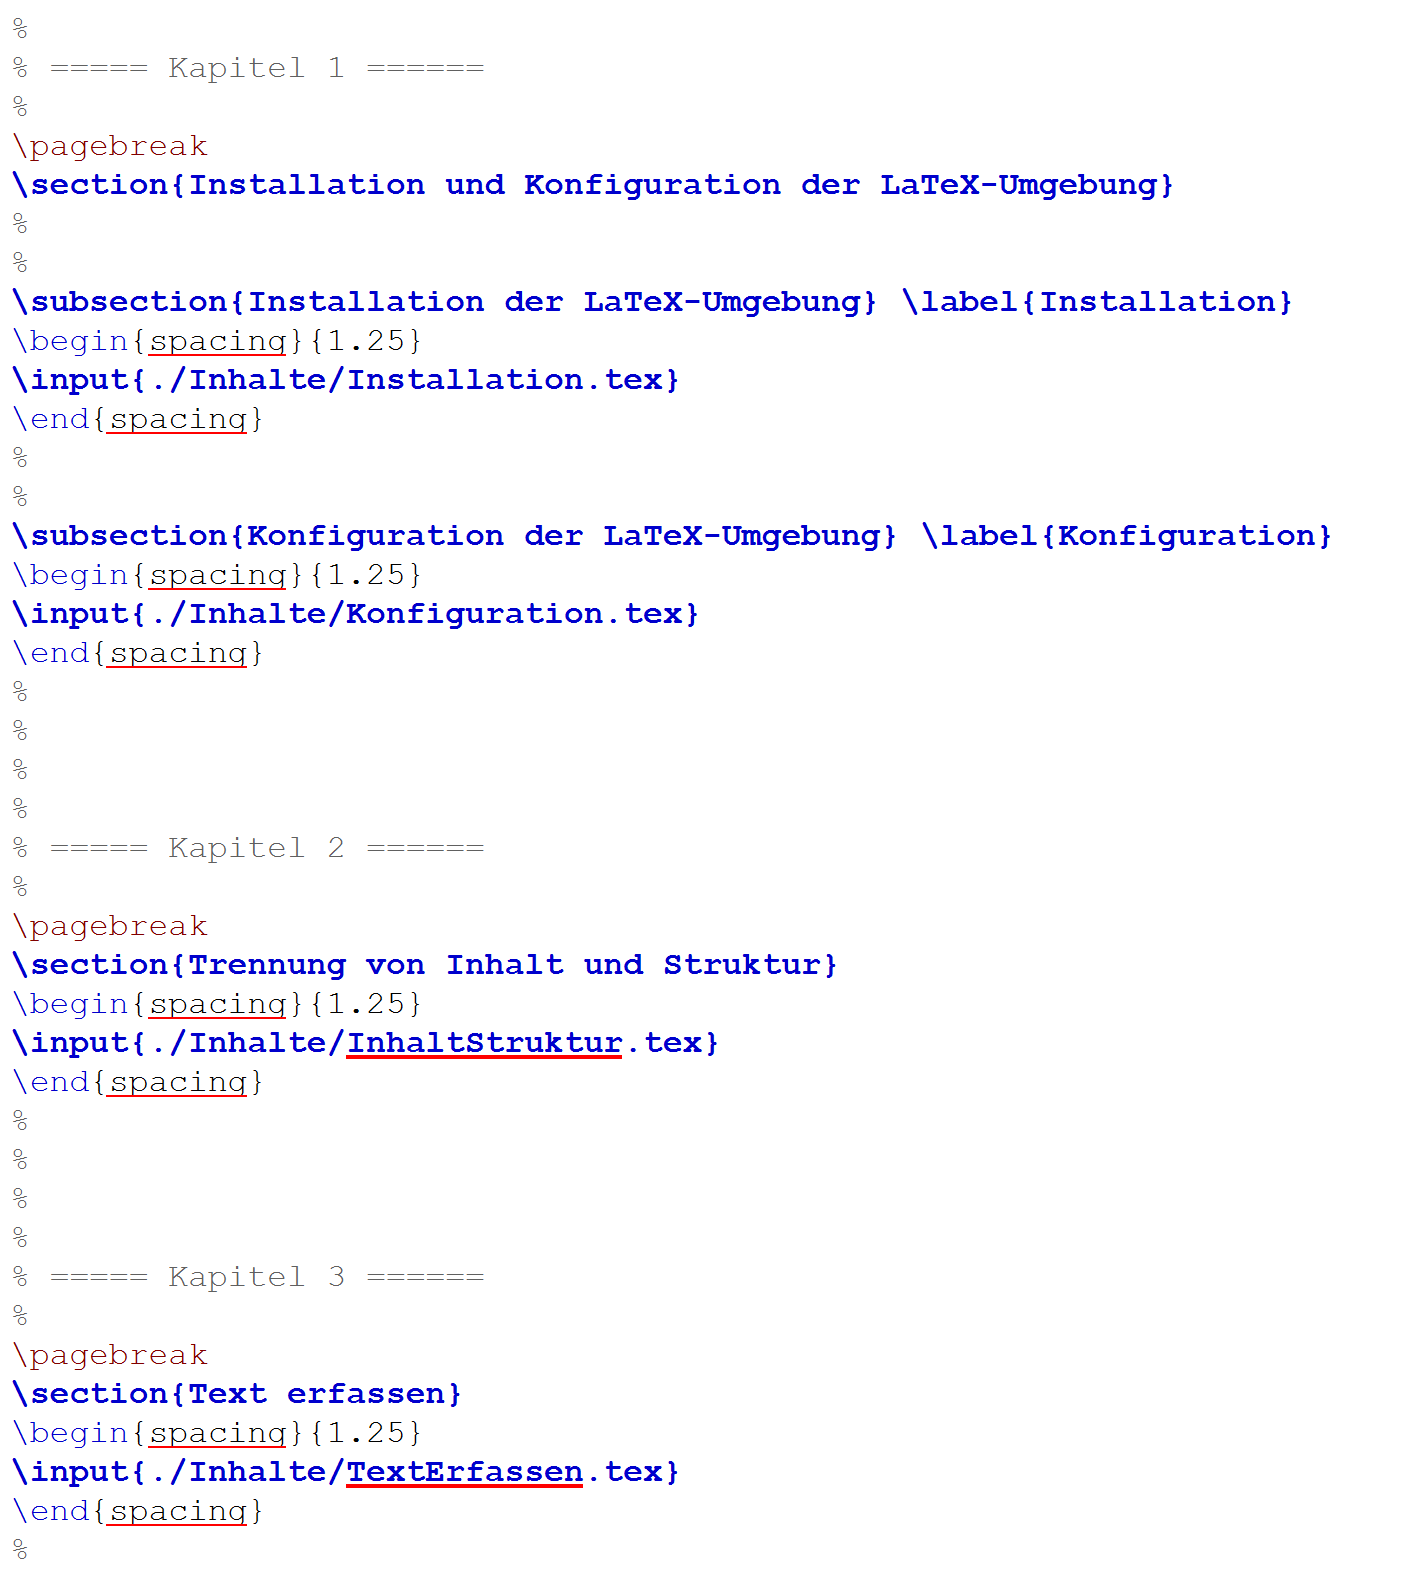
\includegraphics[width=0.9\textwidth]{./Bilder/TextStruktur_1.png}}   % Bild mit Rahmen
  \caption{Kapitel-Struktur des Dokumentes}
  \label{fig:KapitelStruktur}
\end{figure} 

Die eigentlichen fachlichen (Text-) Inhalte der Kapitel sind in separaten \menu{*.tex} Dateien im Verzeichnis \menu{Inhalte} erfasst, die mit dem Befehl \code{\textbackslash{input\{...\}}} eingebunden / eingefügt werden (siehe \cref{fig:KapitelStruktur}: \nameref{fig:KapitelStruktur} auf Seite \pageref{fig:KapitelStruktur}).
